%%%%%%%%%%%%%%%%%%%%%%%%%%%%%%%%%%%%%%%%%%%%%%%%%%%%%%%
% Copyright (c) 2024 Fengming Zhu. All rights reserved.
% Email:        fzhuae@connect.ust.hk
%%%%%%%%%%%%%%%%%%%%%%%%%%%%%%%%%%%%%%%%%%%%%%%%%%%%%%%


\documentclass{beamer}
\usepackage{hyperref}
\usepackage[T1]{fontenc}
\usepackage[numbers]{natbib}
%\UseRawInputEncoding

\usetheme{metropolis}
\definecolor{white}{rgb}{1,1,1}
\beamersetaveragebackground{white}

% other packages
\usepackage{latexsym,amsmath,xcolor,multicol,booktabs,calligra}
\usepackage{amsfonts, amssymb}
\usepackage{graphicx,listings,stackengine}
\usepackage{ulem}

% \usepackage[loadonly]{enumitem}
% \setlistdepth{20}
% \renewlist{itemize}{itemize}{20}

%% Enable only in Xelatex
% \usepackage{pstricks}

\author{Fengming ZHU}  % you can change it to your name
\title{COMP3211 Tutorial 7: Game Theory}
\institute{Department of CSE \\ HKUST \\ {\copyright\ 2024 Fengming Zhu. All rights reserved.}}
\date{Apr. 22\&25, 2024} % you can change it to the latest date


% defs
\def\cmd#1{\texttt{\color{red}\footnotesize $\backslash$#1}}
\def\env#1{\texttt{\color{blue}\footnotesize #1}}
\definecolor{deepblue}{rgb}{0,0,0.5}
\definecolor{deepred}{rgb}{0.6,0,0}
\definecolor{deepgreen}{rgb}{0,0.5,0}
\definecolor{halfgray}{gray}{0.55}

\lstset{
    basicstyle=\ttfamily\small,
    keywordstyle=\bfseries\color{deepblue},
    emphstyle=\ttfamily\color{deepred},    % Custom highlighting style
    stringstyle=\color{deepgreen},
    numbers=left,
    numberstyle=\small\color{halfgray},
    rulesepcolor=\color{red!20!green!20!blue!20},
    frame=shadowbox,
}

{}
\begin{document}

\begin{frame}
    \titlepage
\end{frame}


% \begin{frame}{References}
% \begin{itemize}
%     \item \underline{Main focus}
%     \begin{itemize}
%         \item
%         (SoCS'2013) \textbf{Multi-Agent Path Finding for Self Interested Agents}
%         \cite{bnaya2013multi}
        
%         \item
%         (AAAI'2015) \textbf{Multi-Agent Pathfinding as a Combinatorial Auction}
%         \cite{amir2015multi}

%         \item
%         (Tech report) \textbf{An Empirical Evaluation of a Combinatorial Auction for Solving Multi-Agent Pathfinding Problems}
%     \end{itemize}

%     \item Related
%     \begin{itemize}
%         \item
%         (AAMAS'2019) \textit{Polynomial-Time Multi-Agent Pathfinding with Heterogeneous and Self-Interested Agents}
%         \cite{machida2019polynomial}

%         \item
%         (IROS'2020) \textit{Path Negotiation for Self-interested Multirobot Vehicles in Shared Space}
%         \cite{inotsume2020path}
%     \end{itemize}
% \end{itemize}
% \end{frame}


\begin{frame}{Outline}
    % \tableofcontents[sectionstyle=show,subsectionstyle=show/shaded/hide,subsubsectionstyle=show/shaded/hide]
    \tableofcontents[
    sectionstyle=show,
    subsectionstyle=hide,
    subsubsectionstyle=hide
    ]
\end{frame}


\section{Game Formulation}


\begin{frame}{Formulation}
    \begin{exampleblock}{Normal-Form Games:}
        \begin{itemize}
            \item A set of agents $\mathcal{N} = [1..n]$

            \item Each agent $i$ holds an action set $\mathcal{A}_i$

            \item Each agent $i$ holds an utility function
            $u_i: \mathcal{A}_1 \times \cdots \times \mathcal{A}_n \rightarrow \mathbb{R}$
            
            \item \alert{A Nash equilibrium $(s_1, \cdots, s_n)$,
            $s_i \in \Delta(A_i)$:
            \[
            s_i 
            = BestResponse(s_{-i})
            \triangleq BestResponse(s_1, ...,s_{i-1}, s_{i+1}, \cdots s_n) 
            \]}
            \item Nash's existence theorem:
            Any game with a finite set of players and finite set of strategies has a Nash equilibrium of mixed strategies.
        \end{itemize}
        
    \end{exampleblock}
%    \begin{table}[]
%        \begin{tabular}{c|c|c|}
%        \cline{2-3}
%                                & C    & D    \\ \hline
%        \multicolumn{1}{|c|}{C} & 3, 3 & 1, 5 \\ \hline
%        \multicolumn{1}{|c|}{D} & 5, 1 & 2, 2 \\ \hline
%        \end{tabular}
%        \caption{Prisoner's Delimma}
%    \end{table}
\end{frame}


\subsection{Maximizing Reward v.s. Minimizing Regret}

\begin{frame}{Maximizing Reward v.s. Minimizing Regret}
%\begin{columns}
%    \begin{column}{.5\textwidth}

            \begin{table}[]
                \begin{tabular}{c|c|}
                \cline{2-2}
                                        & Reward \\ \hline
                \multicolumn{1}{|c|}{A} & 100      \\ \hline
                \multicolumn{1}{|c|}{B} & 2      \\ \hline
                \end{tabular}
                % \caption{Single agent with single state}
%            \end{table}
%
%%            \pause
%            \item
%            \begin{table}[]
                \begin{tabular}{c|c|c|}
                \cline{2-3}
                                        & C    & D    \\ \hline
                \multicolumn{1}{|c|}{A} & 100, 3 & $1-\epsilon$, 5 \\ \hline
                \multicolumn{1}{|c|}{B} & 2, 3 & 1, 5 \\ \hline
                \end{tabular}
                % \caption{Nash equilibrium}
%            \end{table}
%
%%            \pause
%%            \item
%            \begin{table}[]
                \begin{tabular}{c|c|c|}
                \cline{2-3}
                                        & C    & D    \\ \hline
                \multicolumn{1}{|c|}{A} & 100, a & $1-\epsilon$, b \\ \hline
                \multicolumn{1}{|c|}{B} & 2, c & 1, d \\ \hline
                \end{tabular}
                % \caption{Minimax regret}
            \end{table}
%    \end{column}    


%    \begin{column}{.5\textwidth}
%\vspace{-2mm}
       \begin{exampleblock}{Definition\footnote{Shoham, Yoav, and Kevin Leyton-Brown. Multiagent systems: Algorithmic, game-theoretic, and logical foundations. Cambridge University Press, 2008.}:}
       $Reward(a_i, a_{-i}) \triangleq u_i(a_i, a_{-i})$
       $Regret(a_i, a_{-1}) \triangleq \max_{a'_i}u_i(a'_i, a_{-i}) - u_i(a_i, a_{-i}) $
       \end{exampleblock}
%    \end{column}
%\end{columns}

\end{frame}


\section{Best Response and Nash Equilibria}

\subsection{Example 1: Network Sharing}

\begin{frame}{Example 1: Network Sharing}
You and your friend share a network and both of you want to download a movie:

- If both of you do that, the network is jammed, and none of you is happy: say both of you value it 2.

- If only one of you do that, the network works perfectly: the one who did that is very happy (5), the other is very unhappy (0).

- If none of you do that, then none of you is very happy but then you can do something together. So let's assign it a value of 3. 
    \begin{table}[]
        \begin{tabular}{c|c|c|}
        \cline{2-3}
                                 & D    & ND    \\ \hline
        \multicolumn{1}{|c|}{D}  & \alert{(2, 2)} & 5, 0 \\ \hline
        \multicolumn{1}{|c|}{ND} & 0, 5 & 3, 3 \\ \hline
        \end{tabular}
%        \caption{Prisoner's Delimma}
    \end{table}
\end{frame}

\subsection{Example 2: Tragedy of The Commons}

\begin{frame}{Example 2: Tragedy of The Commons}
A generalized continuous version:

- n players. Each has the same strategy of downloading $x_i \in [0,1]$ units. But the total bandwidth is only 1. 

- If $\sum_i x_i > 1$, every one gets zero utility.

- Else, player $i$ gets a utility of $x_i(1 - \sum_j x_j)$

\pause
\begin{exampleblock}{Solutoin:}
- Let $t = \sum_{j\neq i} x_i$, then $u_i = x_i(1-t-x_i)$,
max at $x_i=\frac{1-t}{2}$.

- A unique solution for the equations
$\forall i, x_i = \frac{1 - \sum_{j\neq i}x_j}{2}\Rightarrow$ 
$x_i = \frac{1}{n+1}$.

- Total usage $\sum_i x_i = \frac{n}{1+n}$.
Social welfare = $n \cdot \frac{1}{n+1} \frac{1}{n+1} < \frac{1}{n} $.

- But if $\sum_i x_i = 1/2$,
social welfare = $\sum_i x_i (1- \sum_j x_j) = \frac{1}{4}$

- Players are incentivized to \alert{overuse} the resource.
\end{exampleblock}

\end{frame}

\subsection{Example 3: Soccer Penalty Kicks}

\begin{frame}{Example 3: Soccer Penalty Kicks}
    \begin{table}[]
                \begin{tabular}{c|c|c|}
                \cline{2-3}
                        Kicker/Goalie       & Left       & Right    \\ \hline
                \multicolumn{1}{|c|}{Left}  & 0, 1       & 1, 0     \\ \hline
                \multicolumn{1}{|c|}{Right} & 0.75, 0.25 & 0, 1     \\ \hline
                \end{tabular}
                % \caption{Minimax regret}
    \end{table}

\begin{itemize}[<+-| alert@+>]
    \item No pure Nash equilibrium, then try to find a mixed Nash equlibrium.
    \item
    The goalie's strategy is to make the kicker indifferent between kicking left and right.
    Goalie guards left w.p. $p$, for the kicker,
    \[
    (1-p) = 0.75p \Rightarrow p = 4/7
    \]

    \item
    The kicker's strategy is to make the goalie indifferent between guarding left and right.
    Kicker kicks left w.p. $q$, for the guard,
    \[
    q + 0.25(1-q) = (1-q) \Rightarrow q = 3/7
    \] 
\end{itemize}

\end{frame}


\subsection{Example 4: Battle of Sexes}

\begin{frame}{Example 4: Battle of Sexes - Pure NE}
    \begin{table}[]
        \begin{tabular}{c|c|c|}
        \cline{2-3}
                                 & Sports    & Movie    \\ \hline
        \multicolumn{1}{|c|}{Sports}  & 1, 0 & -1, -1 \\ \hline
        \multicolumn{1}{|c|}{Movie} & -1, -1 & 0, 1 \\ \hline
        \end{tabular}
%        \caption{Prisoner's Delimma}
    \end{table}

\center
\alert{Pure-strategy NE: 1. (sports, sports), 2. (movie, movie)}.

What about mixed-strategy NE?
\end{frame}

\begin{frame}{Example 4 con't: Battle of Sexes - All NE}
    \begin{table}[]
        \begin{tabular}{c|c|c|}
        \cline{2-3}
                                 & Sports    & Movie    \\ \hline
        \multicolumn{1}{|c|}{Sports}  & 1, 0 & -1, -1 \\ \hline
        \multicolumn{1}{|c|}{Movie} & -1, -1 & 0, 1 \\ \hline
        \end{tabular}
%        \caption{Prisoner's Delimma}
    \end{table}
    
    \begin{exampleblock}{Best responses:}
    - Suppose the girl plays [q:S, (1-q):M], for the boy to prefer S
    \[
    q - (1-q) \geq -q \Rightarrow q \geq \frac{1}{3} 
    \]
    
    - Suppose the boy plays [p:S, (1-p):M], for the girl to prefer S
    \[
    0 - (1 - p) \geq -p + (1 - p) \Rightarrow p \geq \frac{2}{3}
    \]
    \end{exampleblock}
\end{frame}

\begin{frame}{Example 3 con't: Battle of Sexes - All NE}
\begin{figure}[htpb]
       \centering
       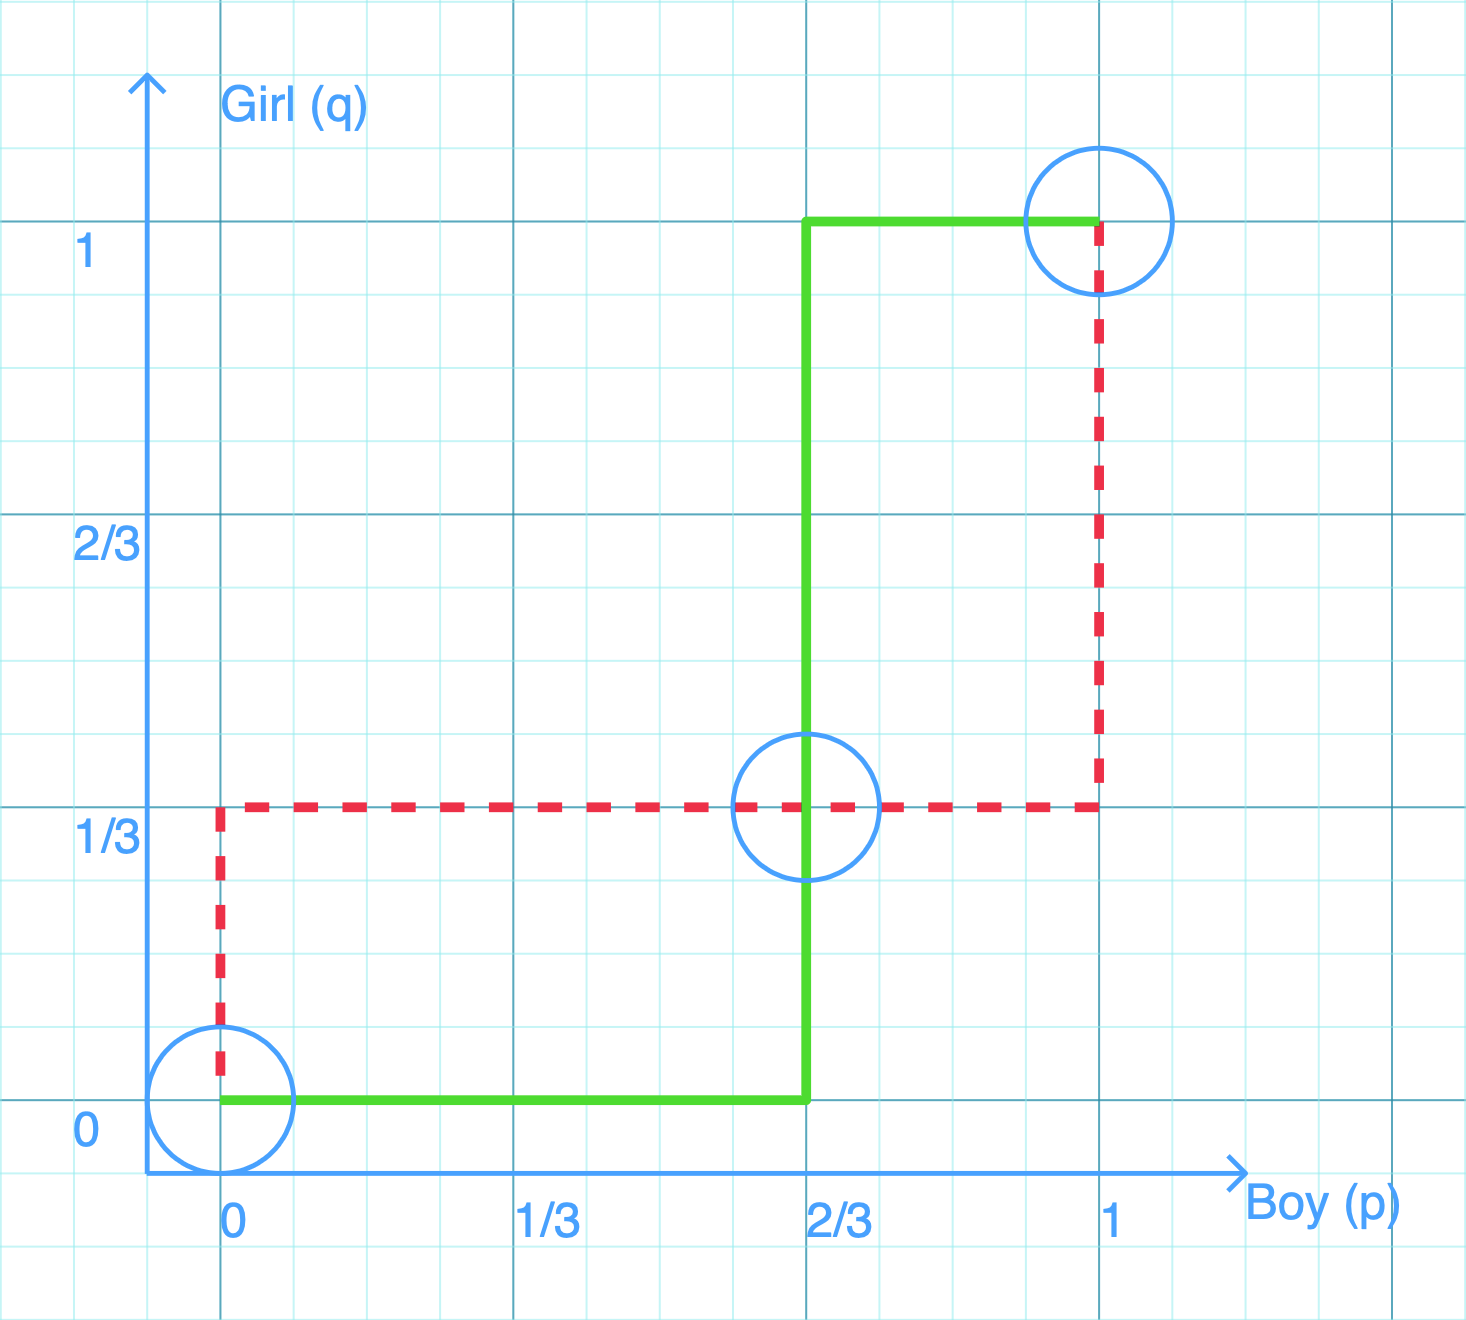
\includegraphics[width=0.5\linewidth]{pic/battleofsexes.png}
       \caption{Best response curve.}  
\end{figure}
Thus, mixed NE: [Boy(2/3:S, 1/3:M), Girl(1/3:S, 2/3:M)].
\end{frame}


\section{Sealed-Bid Auctions}

\begin{frame}{Sealed-Bid Auctions}
	In the lecture, we have discussed two implementations of sealed bid actions: first price auction and second price auction.
\alert{
\begin{enumerate}
	\item First-price: the winner pays his own bid (the highest)
	\item Second-price: the winner pays the second highest bid.
\end{enumerate}
}

For simplicity,	
assume there are two bidders $Alice$ and $Bob$ bidding for one single item. Values that Alice and Bob hold towards the item are $a$ and $b$, respectively. Those values are private information, i.e. $a$ is unknow to Bob and $b$ is unknown to Alice. Let $x$ denote Alice' bid and $y$ denote Bob's bid. Ties will always be broken in favor of Alice.
\end{frame}


\begin{frame}{Sealed-Bid Auctions: First-Price}

Consider first price auction (the highest bidder wins the item and pays the price as she bids).

Assume $a > b$ and Alice somehow knows Bob's valuation $b$, but Bob still has no idea about Alice's valuation $a$. Find a pure Nash 
  equilibrium.
 
\pause\alert{
(x=b, y=b) is the only pure NE, such that Alice can obtain a maximum utility of $a-b > 0$, while Bob has no way to win the item thus no profitable deviation.
}
\end{frame}


\begin{frame}{Sealed-Bid Auctions: First-Price con't}
\small{Assume $a$ and $b$ are independent random variables, both of which are distributed as \texttt{uniform}(0, 1), which is known as common knowledge. Each one's exact value is unknown to the other one, as the original assumption. Find a pure Nash 
  equilibrium. (Hint: try to find the best response for Alice when Bob bids $y=b/2$.)}

\pause\alert{\small{
 Let $y = b/2$, Alice's expected utility will be
$Pr(Alice\ wins) \times (a-x).$
Given $b \sim \texttt{uniform}[0, 1]$, $$Pr(Alice\ wins) = Pr(x \geq b/2) = Pr(b \leq 2x) = 2x.$$
Thus, Alice's expected return will be $2x(a-x)$.
Take the first derivative and set to 0,
\[
\frac{d}{dx} 2x(a-x) = 2a-4x = 0 \Rightarrow x = a/2.
\]
By symmetry, for Alice bidding $a/2$, Bob's best response is also to bid $b/2$.
Hence, $(x=a/2, y=b/2)$ is an NE.
}}
\end{frame}

\begin{frame}{Sealed-Bid Auctions: Revenue Equivalence}
	\begin{exampleblock}{First-price auction:}
	\end{exampleblock}
	
	One-shot income for the auctioneer: $max(a/2, b/2)$
	
	Let $\alpha = max(a/2, b/2)$,
\[
\begin{split}
  Pr[\alpha \leq t]
    & = Pr[max(a/2, b/2) \leq t] \\
    & = Pr[a/2 \leq t] \times Pr[b/2 \leq t] \\
    & = 4t^2 \\
  f(\alpha = t)
    & = d/dt (4t^2) = 8t \\
  E[\alpha]
    & = \int_0^{1/2} t\cdot 8t\cdot dt = 1/3
\end{split}
\]
\end{frame}

\begin{frame}{Sealed-Bid Auctions: Revenue Equivalence}
	\begin{exampleblock}{Second-price auction:}
	\end{exampleblock}
	\alert{It is also proved that (x=a, y=b) is a Nash equilibrium for second price auctions.}
	
	One-shot income for the auctioneer: $min(a, b)$
	
	Let $\beta = min(a, b)$,
\[
\begin{split}
  Pr[\beta \leq t]
    & = Pr[min(a, b) \leq t] \\
    & = 1 - Pr[a > t] \times Pr[b > t] \\
    & = 1- (1-t)^2 \\
  f(\beta = t)
    & = d/dt [1- (1-t)^2] = 2 - 2t \\
  E[\beta]
    & = \int_0^{1} t\cdot (2 - 2t)\cdot dt = 1/3
\end{split}
\]
\end{frame}




%
%\section{Mechanism Design}
%
%
%\begin{frame}{Mechanism Design with Money - Auctions}
%    \begin{exampleblock}{Auction:}
%        \begin{itemize}[<+-| alert@+>]
%            \item First price auction: the highest bidder wins and pays her bid
%            \[
%                u_i(b_1, \cdots, b_i, \cdots, b_n) = 
%                \begin{cases}
%                    v_i - b_i & \text{, i wins the item} \\
%                    0 - 0 & \text{, otherwise}
%                \end{cases}
%            \]
%
%            \item Second price auction: the highest bidder wins but pays the second highest bid
%            \[
%                u_i(b_1, \cdots, b_i, \cdots, b_n) = 
%                \begin{cases}
%                    v_i - \max {(\vec{b} \backslash \{b_i\})} & \text{, i wins the item} \\
%                    0 - 0 & \text{, otherwise}
%                \end{cases}
%            \]
%
%            \item Second price auction is truthful!
%        \end{itemize}
%    \end{exampleblock}
%\end{frame}
%
%
%\begin{frame}{Exercise: Modified First Price Aution}
%There are 3 agents who bid for an item under a modified 1st price auction described below. It's a common knowledge that everyone's
%value of the item is 5, and they can bid any price in the set $\{0,1,2,3,4,5\}$.
%The modified 1st price auction is as follows: 
%
%1. if there is no tie, then the higest bidder wins the item and pay for what she bid for it;
%
%2. if two of them tie for the highest bid, then the one who bid a lower value wins the item and pay for what she bid for it; 
%
%3. if all of them bid the same price, then there is no winner. 
%
%Assume the usual risk neutral utility function. 
%Formulate this auction as a game in normal form and compute all its pure Nash equilibria, if any.
%\end{frame}
%
%
%\begin{frame}{Exercise: Modified First Price Aution - Solution}
%    \begin{enumerate}
%    \item Players $N=\{1, 2, 3\}$.
%    
%    \item Actions $A = \{0, 1, \cdots , 5\}$.
%    
%    \item Utility functions $u_i: A^3 \mapsto \{0, 1, \cdots , 5\}$, calculated as follows ($b_{-i}$ denotes the other two bids),
%    \[
%    u_i(b_i, b_{-i}) = 
%    \begin{cases}
%    5 - b_i &, \text{if } b_i > \max(b_{-i}) \\
%    0 &, \text{if } b_i = \max(b_{-i}) \\
%    0 &, \text{if } b_i < \max(b_{-i}) \text{ and } noTie(b_{-i})\\
%    5 - b_i &, \text{if } b_i < \max(b_{-i}) \text{ and } Tie(b_{-i})\\
%    \end{cases}
%    \]
%\end{enumerate}
%
%\pause
%All bidding profiles like
%$(5,5,0), (5, i<5, j<5), (4,4,0), (4, l<4, k<4)$ permuted over three players are pure strategy NEs.
%
%\end{frame}


% \begin{frame}{Exercise:}
%     \begin{itemize}
%         \item Think of an integer between [1..99], send me in a private chat.

%         \item The one whose number is closest to $\lceil \frac{2}{3} AVG(allNumbers) \rceil$ win the game.  
%     \end{itemize}
% \end{frame}



% \begin{frame}{Cooperative v.s. Self-interested}

% \begin{exampleblock}{Cooperative agents:}
% \begin{itemize}
%     \item Input: {a weighted graph, N agents (starts/goals)}
    
%     \item Objective: {minimize global cost}
% \end{itemize}
% \end{exampleblock}

% \pause
% \begin{exampleblock}{Self-interested agents:}
% \begin{itemize}
%     \item Objective: {minimize \textbf{individual cost}}

%     \pause
%     \item A naïve way: {each schedule herself individually, resolve conflicts randomly}
% \end{itemize}
% \end{exampleblock}

% \end{frame}


% \begin{frame}{Relation with Traffic Control}

% \begin{exampleblock}{Traffic flow network:}
% \begin{itemize}
%     \item Continuous flow along edges, causing certain \alert{delays}

%     \item Selfish routing is proved to be non-optimal

%     \item Toll/taxation mechanisms are usaully used.

%     \item Sometimes coincides with congestion games (a classical \alert{potential game}) 
% \end{itemize}
% \end{exampleblock}

% \end{frame}



% \begin{frame}{An Example}

% % \begin{figure}[htpb]
% %         \centering
% %         \includegraphics[width=0.6\linewidth]{pic/tax_eg.png}
% % \end{figure}

% \begin{columns}
%     \begin{column}{.5\textwidth}
%     \centering
%         \underline{Selfish routing} \\
%         a1: \{S1, \_, C, G1\} \\
%         a2: \{S2, C, G2\} \\
%         a3: \{S3, \_, C, G3\} \\
%         $\Rightarrow (3+\alert{1}) + 2 + (3+\alert{2}) = 11$
%     \end{column}    

%     \pause
%     \begin{column}{.5\textwidth}
%     \centering
%         \underline{With taxation} \\
%         a1: \{S1, left-hand, G1\} \\
%         a2: \{S2, C, G2\} \\
%         a3: \{S3, right-hand, G3\} \\
%         $\Rightarrow \alert{4} + 2 + \alert{4} = 10$
%     \end{column}
% \end{columns}

% \end{frame}


% \begin{frame}{Formally}

% \begin{exampleblock}{Key idea:}
% \begin{itemize}
%     \item Assign each edge/vertex a tax (penalty)

%     \item Individually minimizes $\hat{c}(P_i) = c(P_i) + T(P_i)$

%     \pause[2]
%     \item \alert{$\Rightarrow$ Iterative Taxation Framework}
%     % \begin{figure}[htpb]
%     %     \centering
%     %     \includegraphics[width=0.8\linewidth]{pic/ITF.png}
%     % \end{figure}

%     \pause[3]
%     \item Implementations: 1) Exhaustive 2) Monte-Carlo
% \end{itemize}
% \end{exampleblock}

% \end{frame}


% \begin{frame}{Evaluation -- toy example}

% % \begin{figure}[htpb]
% %         \centering
% %         \includegraphics[width=1\linewidth]{pic/result_3x3.png}
% %         \caption{EITA (exhaustive iterative taxation algorithm),
% %                 MC-ITA (Monte-Carlo iterative taxation algorithm),
% %                 Lowerbound (global optimum)} 
% % \end{figure}

% \end{frame}


% \begin{frame}{Evaluation -- large scale}

% \begin{columns}
%     \begin{column}{.65\columnwidth}
%         % \begin{figure}[htpb]
%         %     \centering
%         %     \includegraphics[width=1\linewidth]{pic/result_den520.png}
%         %     \caption{den520d for 10 agents}
%         % \end{figure}
%     \end{column}

%     \begin{column}{.35\columnwidth}
%         % \begin{figure}[htpb]
%         %     \centering
%         %     \includegraphics[width=1\linewidth]{pic/den520d.pdf}
%         %     \caption{den520d -- dimension ($257\times 256$), \#states (28178)}
%         % \end{figure}
%     \end{column}
% \end{columns}

% \end{frame}


% \begin{frame}{Drawbacks}

% \begin{itemize}
%     \item Not guaranteed to minimize global cost (maximize social welfare)

%     \item Not strategyproof: agents could misreport their starts/goals

%     \item Agents are restricted to be homogeneous

%     \pause
%     \item \alert{Let's seek help from auctions!}
% \end{itemize}

% \end{frame}



% \begin{frame}{Conventional Combinatorial Auction}

% \begin{exampleblock}{Preliminaries}
%     \begin{itemize}
%         \item Agents: $N = \{1, \cdots, n\}$

%         \item Actioned items: $M = \{1, \cdots, m\}$

%         \item Valuation function for each agent $v_i: 2^M \mapsto \mathbb{R}$

%         \pause
%         \alert{
%         \item A mechanism (with monetary transfer) is a pair of
%         \begin{itemize}
%             \item a social choice function $f: V_1 \times \cdots \times V_n \mapsto A$
            
%             \item a vector of payments functions $p_1, \cdots, p_n$, where $p_i: V_1 \times \cdots \times V_n \mapsto \mathbb{R}$
%         \end{itemize}}
%     \end{itemize}
% \end{exampleblock}

% \end{frame}


% \begin{frame}{Reduce to CA}

%     % \begin{figure}[htpb]
%     %     \centering
%     %     \includegraphics[width=1\linewidth]{pic/reduction.png}
%     % \end{figure}

%     \pause
%     \begin{exampleblock}{Derived valuation function:}
%     \begin{itemize}[<+-| alert@+>]
%         \item $v_i(p) = val(g_i) - c(p)$

%         \item Turns out $val(g_i) := max_c \times n$ [constant]
%     \end{itemize}
%     \end{exampleblock}

% \end{frame}


% \begin{frame}{Strategic Manipulation}

%     % \begin{figure}[htpb]
%     %     \centering
%     %     \includegraphics[width=0.4\linewidth]{pic/ca_eg.png}
%     %     \caption{Assuming $v_i(g_i) = 10$}
%     % \end{figure}

%     \begin{exampleblock}{A centralized yet not strategyproof mechanism:}
%     \begin{itemize}[<+-| alert@+>]
%         \item If a1 and a2 report truthfully,
%             \begin{itemize}
%                 \item a1 gets 10-(1.5+1), a2 gets 10-(1+1)
%             \end{itemize}

%         \item If a1 misreports (s1, X) = 1.8,
%             \begin{itemize}
%                 \item a1 gets 10-(1+1), a2 gets 10-(1.7+1)
%             \end{itemize}
%     \end{itemize}
%     \end{exampleblock}

% \end{frame}


% \begin{frame}{Strategic Manipulation}

%     % \begin{figure}[htpb]
%     %     \centering
%     %     \includegraphics[width=0.3\linewidth]{pic/ca_eg.png}
%     %     \caption{Assuming $v_i(g_i) = 10$}
%     % \end{figure}

%     \begin{exampleblock}{The well-known VCG mechanism:}
%     \begin{itemize}[<+-| alert@+>]
%         \item Payment := the harm you did to others' social welfare

%         \item If a1 and a2 report truthfully,
%             \begin{itemize}
%                 \item a1 gets 10-(1.5+1)-0 = 7.5, a2 gets 10-(1+1)-0.5
%             \end{itemize}

%         \item If a1 misreports (s1, X) = 1.8,
%             \begin{itemize}
%                 \item a1 gets 10-(1+1)-0.7 = 7.3, a2 gets 10-(1.7+1)-0
%             \end{itemize}
%     \end{itemize}
%     \end{exampleblock}

% \end{frame}


% \begin{frame}{Computational Issues}

% \begin{itemize}
%     \item In sealed-bid auctions, such as VCG, each agent needs to bid over all bundles that it may be interested in. 

%     \item In MAPF, this means that an agent $i$ would need to find all paths from $s_i$ to $g_i$ and place bids on them.

%     \item The number of paths between two vertices in a graph may be exponential in the path length.

%     \item Moreover, to find an allocation that maximizes its revenue, the auctioneer will need to check the cross product of these potentially exponential number of bids.

%     \pause
%     \item \alert{Interative combinatorial auction (Parkes 2006)}
% \end{itemize}

% \end{frame}


% \begin{frame}{Iterative Combinatorial Auction}

% \begin{exampleblock}{Basic framework (\textit{iBundle}):}
% \begin{itemize}
%     \item Bidding

%     \item Winner determination

%     \item Price update
% \end{itemize}
% \end{exampleblock}

% \end{frame}


% \begin{frame}{iBundle -- Bidding}

%     % \begin{figure}[htpb]
%     %     \centering
%     %     \includegraphics[width=0.8\linewidth]{pic/bidding.png}
%     % \end{figure}

%     \begin{exampleblock}{Bidding:}
%         \begin{itemize}[<+-| alert@+>]
%             \item Agents place \texttt{XOR} bids on their \underline{desired} bundles.

%             \item Minimize $cost(p) + ask(p)$

%             \item $a_3$ bids $[<F, t_1>, <D, t_2>, <G, t_3>, <E, t_4>, <I, t_5>]; [<F, t_1>, <D, t_2>, <C, t_3>, <E, t_4>, <I, t_5>]$.

%             \item Myopic best response is a dominant strategy
%         \end{itemize}
%     \end{exampleblock}

% \end{frame}


% \begin{frame}{iBundle -- Winner Dermination}

%     % \begin{figure}[htpb]
%     %     \centering
%     %     \includegraphics[width=0.8\linewidth]{pic/bidding.png}
%     % \end{figure}

%     \begin{exampleblock}{Winner determination:}
%         \begin{itemize}[<+-| alert@+>]
%             \item Determine a provisional allocation

%             \item To maximizes seller's revenue and include more non-conflicting agents

%             \item $a_1$ gets $[<A, t_1>, <C, t_2>]$, $a_3$ gets $[<F, t_1>, <D, t_2>, <G, t_3>, <E, t_4>, <I, t_5>]$
%         \end{itemize}
%     \end{exampleblock}

% \end{frame}


% \begin{frame}{iBundle -- Price Update}

%     % \begin{figure}[htpb]
%     %     \centering
%     %     \includegraphics[width=0.8\linewidth]{pic/bidding.png}
%     % \end{figure}

%     \begin{exampleblock}{Price update:}
%         \begin{itemize}[<+-| alert@+>]
%             \item Initial prices for all bundles are 0

%             \item Bundles that ``unhappy'' agents bid on are raised by $\epsilon$

%             \item In MAPF, sufficient to set $\epsilon = \min(c_e)$

%             \item $a_2$ is unhappy, prices of paths of $MDD_2^3$ are raised by 1
%         \end{itemize}
%     \end{exampleblock}

% \end{frame}


% \begin{frame}{Evaluation}
%     % \begin{figure}[htpb]
%     %     \includegraphics[width=0.6\linewidth]{pic/ca_small}
%     % \end{figure}
% \end{frame}


% \begin{frame}{Evaluation}
%     % \begin{figure}[htpb]
%     %     \includegraphics[width=0.6\linewidth]{pic/ca_large}
%     % \end{figure}
% \end{frame}



% %%%%%%%%%% part 4 %%%%%%%%%%


% \begin{frame}{Insights}

% \begin{itemize}[<+-| alert@+>]
%     \item Consider heterogeneous and self-interested agents

%     \item Still, complexity issues due to the combinatorial nature

%     \item One-parameter agents, e.g. fuel consumption  
%     \begin{itemize}
%         \item Seems poly-time strategyproof mechanism exists \cite{machida2019polynomial}
%     \end{itemize}

%     \item Negotiation and bargaining on paths\cite{inotsume2020path}
% \end{itemize}

% \end{frame}


% \begin{frame}[allowframebreaks]
%     \bibliography{ref}
%     \bibliographystyle{alpha}
%     % If too many references, use this command to resize:
%     % \tiny\bibliographystyle{alpha}
% \end{frame}


\begin{frame}
    \begin{center}
        {\Huge\calligra Thanks!}
    \end{center}
\end{frame}


% \begin{frame}{A Running Example}
    % \begin{figure}[htpb]
    %     \centering
    %     \includegraphics[width=0.5\linewidth]{pic/mapf_ca_eg.png}
        
    %     \pause
    %     \includegraphics[width=1\linewidth]{pic/mapf_ca_proc_1.png}
        
    %     \pause
    %     \includegraphics[width=1\linewidth]{pic/mapf_ca_proc_2.png}
        
    %     \pause
    %     \includegraphics[width=1\linewidth]{pic/mapf_ca_proc_3.png}
    % \end{figure}
% \end{frame}

% \begin{frame}{Sequential $\to$ Decentralized}
%     \begin{block}{}
%         \begin{figure}[htpb]
%             \centering
%             \includegraphics[width=0.3\linewidth]{pic/gradient.png}
%         \end{figure}
%     \end{block}

%     \pause
%     \begin{columns}
%         \begin{column}{.5\textwidth}
%         \centering
%             \begin{exampleblock}{Sequential update}
%                 \begin{itemize}
%                     \item
%                     For $i = 1 \to k$,
%                     \begin{itemize}
%                         \item While not converge,
%                         \begin{itemize}
%                             \item \texttt{Gradient ascent}
%                         \end{itemize}
%                     \end{itemize}
%                 \end{itemize}
%             \end{exampleblock}
%         \end{column}    

%         \pause
%         \begin{column}{.5\textwidth}
%         \centering
%             \begin{exampleblock}{Decentralized update}
%                 \begin{itemize}
%                     \item
%                     For every $i \in [1..k]$,
%                     \begin{itemize}
%                         \item While not converge,
%                         \begin{itemize}
%                             \item \texttt{Gradient ascent}
%                             \item \alert{\texttt{Broadcast}$({v}_i)$}
%                         \end{itemize}
%                     \end{itemize}
%                 \end{itemize}
%             \end{exampleblock}
%         \end{column}
%     \end{columns}
% \end{frame}


% \begin{frame}{Issues}
%     \begin{columns}
%         \begin{column}{.3\columnwidth}
%             \begin{figure}[htpb]
%                 \centering
%                 \includegraphics[width=1.1\linewidth]{pic/bias.png}
%             \end{figure}
%         \end{column}

%         \begin{column}{.7\columnwidth}
%             \begin{itemize}[<+-| alert@+>]
%                 \item 
%                 MNIST for minibatch sizes of 1024 (top), 512 (middle), and 256 (bottom)

%                 \item
%                 The figure shows the performance of EigenGame degrades in the low batch size regime.

%                 % \item
%                 % Because we use the same minibatch for all inner products in the gradient which contains products and ratios of random variables.

%                 \item Current hardware easily supports batches of 1024 for MNIST and 128 for IMAGENET

%                 \item \underline{\textbf{But still, can we reduce the bias?}}
%             \end{itemize}
%         \end{column}
%     \end{columns}
% \end{frame}


% \begin{frame}{Figure and Column}
%     % From thuthesis user guide.
%     \begin{minipage}[c]{0.3\linewidth}
%     %%% DO NOT USE PSTricks in pdflatex
% %         \psset{unit=0.8cm}
% %         \begin{pspicture}(-1.75,-3)(3.25,4)
% %             \psline[linewidth=0.25pt](0,0)(0,4)
% %             \rput[tl]{0}(0.2,2){$\vec e_z$}
% %             \rput[tr]{0}(-0.9,1.4){$\vec e$}
% %             \rput[tl]{0}(2.8,-1.1){$\vec C_{ptm{ext}}$}
% %             \rput[br]{0}(-0.3,2.1){$\theta$}
% %             \rput{25}(0,0){%
% %             \psframe[fillstyle=solid,fillcolor=lightgray,linewidth=.8pt](-0.1,-3.2)(0.1,0)}
% %             \rput{25}(0,0){%
% %             \psellipse[fillstyle=solid,fillcolor=yellow,linewidth=3pt](0,0)(1.5,0.5)}
% %             \rput{25}(0,0){%
% %             \psframe[fillstyle=solid,fillcolor=lightgray,linewidth=.8pt](-0.1,0)(0.1,3.2)}
% %             \rput{25}(0,0){\psline[linecolor=red,linewidth=1.5pt]{->}(0,0)(0.,2)}
% % %           \psRotation{0}(0,3.5){$\dot\phi$}
% % %           \psRotation{25}(-1.2,2.6){$\dot\psi$}
% %             \psline[linecolor=red,linewidth=1.25pt]{->}(0,0)(0,2)
% %             \psline[linecolor=red,linewidth=1.25pt]{->}(0,0)(3,-1)
% %             \psline[linecolor=red,linewidth=1.25pt]{->}(0,0)(2.85,-0.95)
% %             \psarc{->}{2.1}{90}{112.5}
% %             \rput[bl](.1,.01){C}
% %         \end{pspicture}
%     \end{minipage}\hspace{1cm}
%     \begin{minipage}{0.5\linewidth}
%         \medskip
%         %\hspace{2cm}
%         \begin{figure}[h]
%             \centering
%             \includegraphics[height=.4\textheight]{pic/dtmf.pdf}
%         \end{figure}
%     \end{minipage}
% \end{frame}

% \begin{frame}[fragile]{\LaTeX{} Commands}
%     \begin{exampleblock}{Commands}
%         \centering
%         \footnotesize
%         \begin{tabular}{llll}
%             \cmd{chapter} & \cmd{section} & \cmd{subsection} & \cmd{paragraph} \\
%             Chapter & Section & Subsection & Paragraph \\\hline
%             \cmd{centering} & \cmd{emph} & \cmd{verb} & \cmd{url} \\
%             Centre Align & Emphasis & Verbatim & Hyperlink \\\hline
%             \cmd{footnote} & \cmd{item} & \cmd{caption} & \cmd{includegraphics} \\
%             Foodnote & Item & Caption & FigP\&Pic \\\hline
%             \cmd{label} & \cmd{cite} & \cmd{ref} \\
%             Label & Citing & Referring\\\hline
%         \end{tabular}
%     \end{exampleblock}
%     \begin{exampleblock}{Environment Command}
%         \centering
%         \footnotesize
%         \begin{tabular}{lll}
%             \env{table} & \env{figure} & \env{equation}\\
%             Table & Figure & Equation \\\hline
%             \env{itemize} & \env{enumerate} & \env{description}\\
%             Bullets & Numbering & Description \\\hline
%         \end{tabular}
%     \end{exampleblock}
% \end{frame}

% \begin{frame}[fragile]{\LaTeX{} Environment Command Samples}
%     \begin{minipage}{0.5\linewidth}
% \begin{lstlisting}[language=TeX]
% \begin{itemize}
%   \item A \item B
%   \item C
%   \begin{itemize}
%     \item C-1
%   \end{itemize}
% \end{itemize}
% \end{lstlisting}
%     \end{minipage}\hspace{1cm}
%     \begin{minipage}{0.3\linewidth}
%         \begin{itemize}
%             \item A
%             \item B
%             \item C
%             \begin{itemize}
%                 \item C-1
%             \end{itemize}
%         \end{itemize}
%     \end{minipage}
%     \medskip
%     \pause
%     \begin{minipage}{0.5\linewidth}
% \begin{lstlisting}[language=TeX]
% \begin{enumerate}
%   \item Class 1 
%   \item Class 2
%   \item Class 2
%   \begin{itemize}
%     \item[n+e] Student 1
%   \end{itemize}
% \end{enumerate}
% \end{lstlisting}
%     \end{minipage}\hspace{1cm}
%     \begin{minipage}{0.3\linewidth}
%         \begin{enumerate}
%             \item Class 1
%             \item Class 2
%             \item Class 3
%             \begin{itemize}
%                 \item[n+e] Student 1
%             \end{itemize}
%         \end{enumerate}
%     \end{minipage}
% \end{frame}

% \begin{frame}[fragile]{\LaTeX{} Equations}
%     \begin{columns}
%         \begin{column}{.55\textwidth}
% \begin{lstlisting}[language=TeX]
% $V = \frac{4}{3}\pi r^3$

% \[
%   V = \frac{4}{3}\pi r^3
% \]

% \begin{equation}
%   \label{eq:vsphere}
%   V = \frac{4}{3}\pi r^3
% \end{equation}
% \end{lstlisting}
%         \end{column}
%         \begin{column}{.4\textwidth}
%             $V = \frac{4}{3}\pi r^3$
%             \[
%                 V = \frac{4}{3}\pi r^3
%             \]
%             \begin{equation}
%                 \label{eq:vsphere}
%                 V = \frac{4}{3}\pi r^3
%             \end{equation}
%         \end{column}
%     \end{columns}
%     \begin{itemize}
%         \item Check more \href{https://en.wikipedia.org/wiki/Help:Displaying_a_formula}{\color{purple}{Here}}
%     \end{itemize}
% \end{frame}

% \begin{frame}[fragile]
%     \begin{columns}
%         \column{.6\textwidth}
% \begin{lstlisting}[language=TeX]
% \begin{table}[htbp]
%   \caption{Definition}
%   \label{tab:number}
%   \centering
%   \begin{tabular}{cl}
%     \toprule
%     Word & Definition \\
%     \midrule
%     1 & 4.0 \\
%     2 & 3.7 \\
%     \bottomrule
%   \end{tabular}
% \end{table}
% Check definition of 
% Equation~(\ref{eq:vsphere}) 
% in Table~\ref{tab:number}。
% \end{lstlisting}
%         \column{.4\textwidth}
%         \begin{table}[htpb]
%             \centering
%             \caption{Definition}
%             \label{tab:number}
%             \begin{tabular}{cl}\toprule
%                 Eq. & Def. \\\midrule
%                 1 & 4.0\\
%                 2 & 3.7\\\bottomrule
%             \end{tabular}
%         \end{table}
%         \normalsize Please check the definition of Equation~(\ref{eq:vsphere}) in Table~\ref{tab:number}
%     \end{columns}
% \end{frame}

% \begin{frame}{Plotting}
%     \begin{itemize}
%         \item Vector: eps, ps, pdf
%         \begin{itemize}
%             \item METAPOST, pstricks, pgf $\ldots$
%             \item Xfig, Dia, Visio, Inkscape $\ldots$
%             \item Export Matlab / Excel as pdf
%         \end{itemize}
%         \item Bitmap: png, jpg, tiff $\ldots$
%         \begin{itemize}
%             \item Avoiding using bitmaps 
%         \end{itemize}
%     \end{itemize}
%     \begin{figure}[htpb]
%         \centering
%         \includegraphics[width=0.2\linewidth]{pic/QUT_Logo_CMYK.jpg}
%         \caption{This is a Bitmaps}
%     \end{figure}
% \end{frame}

\end{document}